\documentclass[12pt,a4paper]{article}

\usepackage[T1]{fontenc}
\usepackage[utf8]{inputenc}
\usepackage{mathptmx}
\usepackage[a4paper,top=2.5cm,bottom=2.5cm,left=3cm,right=2.5cm]{geometry}
\usepackage{setspace}
\usepackage{etoolbox}
\usepackage{titlesec}
\usepackage{fancyhdr}
\usepackage{graphicx}
\usepackage{pdflscape}
\usepackage{booktabs}
\usepackage{tabularx}
\usepackage{longtable}
\usepackage{array}
\usepackage{float}
\usepackage{amsmath}
\usepackage{xcolor}
\usepackage{listings}
\usepackage{enumitem}
\usepackage{url}
\usepackage{tikz}
\usetikzlibrary{calc, positioning, shapes.geometric, arrows.meta}
\usepackage[colorlinks=true,linkcolor=black,citecolor=black,urlcolor=blue]{hyperref}

\newcommand{\projtitle}{Deep Learning-Based Real-Time Ergonomic Posture Monitoring System}
\newcommand{\stuA}{Pranava Pai N}
\newcommand{\stuB}{Ashish Shenoy K}
\newcommand{\stuC}{Krrish Raj Kushagray}
\newcommand{\usnA}{4SF23CS147}
\newcommand{\usnB}{4SF23CS0XX}
\newcommand{\usnC}{4SF23CS089}

\newcommand{\declimage}{images/combined.png}
\newcommand{\placeholder}[1]{\textcolor{red}{[#1]}}
\newcolumntype{Y}{>{\raggedright\arraybackslash}X}

\renewcommand{\thesection}{\arabic{section}}
\titleformat{\section}{\fontsize{16}{20}\selectfont\bfseries}{\thesection.}{0.6em}{}
\titleformat{\subsection}{\fontsize{14}{18}\selectfont\bfseries}{\thesubsection}{0.6em}{}
\titleformat{\subsubsection}{\fontsize{12}{15}\selectfont\bfseries}{\thesubsubsection}{0.6em}{}
\titlespacing*{\section}{0pt}{0pt}{14pt}
\titlespacing*{\subsection}{0pt}{14pt}{6pt}
\titlespacing*{\subsubsection}{0pt}{10pt}{4pt}

\onehalfspacing
\setlength{\parindent}{0pt}
\setlength{\parskip}{6pt}
\setlist{itemsep=2pt,topsep=2pt,parsep=0pt}
\AtBeginEnvironment{table}{\singlespacing}
\AtBeginEnvironment{figure}{\singlespacing}
\AtBeginEnvironment{lstlisting}{\singlespacing}

\pagestyle{fancy}
\fancyhf{}
\fancyfoot[R]{\small\thepage}
\renewcommand{\headrulewidth}{0.4pt}
\renewcommand{\footrulewidth}{0.4pt}
\setlength{\headheight}{14.5pt}

\definecolor{codegreen}{rgb}{0,0.5,0}
\definecolor{codegray}{rgb}{0.5,0.5,0.5}
\definecolor{backcolour}{rgb}{0.96,0.96,0.94}
\lstdefinestyle{mystyle}{
    backgroundcolor=\color{backcolour},
    commentstyle=\color{codegreen},
    keywordstyle=\color{blue},
    numberstyle=\tiny\color{codegray},
    basicstyle=\ttfamily\footnotesize,
    breaklines=true, breakatwhitespace=false,
    captionpos=b, keepspaces=true,
    numbers=left, numbersep=5pt,
    showspaces=false, showstringspaces=false, tabsize=2,
    xleftmargin=1.5em, aboveskip=8pt, belowskip=6pt
}
\lstset{style=mystyle}

\newcommand{\logo}[2]{\IfFileExists{#1}{\includegraphics[height=#2]{#1}}{\fbox{\rule{0pt}{#2}\rule{#2}{0pt}}}}

\newcommand{\snap}[2]{%
  \IfFileExists{#1}{\includegraphics[width=0.85\textwidth]{#1}}{%
  \fbox{\parbox[c][5cm][c]{0.8\textwidth}{\centering\textcolor{red}{Insert screenshot:}\\ #2}}}}

\newcommand{\rubricpage}[2]{%
\begin{landscape}
\thispagestyle{empty}
\begingroup
\singlespacing\small
\centering
{\fontsize{14}{18}\selectfont\bfseries EVALUATION RUBRICS}\\[10pt]
\raggedright
\textbf{Name:} #1 \hfill \textbf{USN:} #2\par
\vspace{8pt}
\renewcommand{\arraystretch}{1.3}
\setlength{\tabcolsep}{5pt}
\noindent\begin{tabularx}{\linewidth}{|c|>{\raggedright\arraybackslash}p{2.6cm}|Y|Y|Y|Y|p{1.5cm}|}
\hline
\textbf{Sl. No.} & \textbf{Evaluation Criteria} & \textbf{Excellent (4)} & \textbf{Good (3)} & \textbf{Satisfactory (2)} & \textbf{Poor (1)} & \textbf{Marks}\\
\hline
1 & Problem Definition \& Objectives & Problem is clearly defined, relevant, and objectives are specific and measurable & Problem and objectives are clear with minor gaps & Problem is partially defined; objectives need improvement & Problem/objectives are unclear & \\[20pt]
\hline
2 & Technical Approach \& Implementation & Appropriate methodology, algorithms/tools used effectively; implementation is complete & Appropriate technical approach with minor issues & Basic implementation with limited technical depth & Incomplete or inappropriate implementation & \\[20pt]
\hline
3 & Innovation / Application / Problem Solving & Demonstrates strong originality, creativity, and effective solution to the identified problem & Shows some innovation and good problem solving & Limited innovation; mostly conventional approach & No significant innovation/problem-solving & \\[20pt]
\hline
4 & Results, Testing \& Analysis & Results are clearly presented, thoroughly tested, and critically analyzed using suitable measures & Results presented with adequate testing and analysis & Basic results and limited testing/analysis & Results are incomplete or unsupported & \\[20pt]
\hline
5 & Documentation, Presentation \& Viva & Well-structured report, clear presentation, excellent communication and confident viva & Good documentation, presentation and satisfactory viva & Adequate documentation/ presentation with limited clarity & Poor documentation, presentation or viva & \\[20pt]
\hline
 & \textbf{Total} & & & & & \\[12pt]
\hline
\end{tabularx}
\endgroup
\end{landscape}
}
\begin{document}

\newgeometry{top=2.2cm,bottom=2.2cm,left=2.5cm,right=2.5cm}
\begin{titlepage}
\thispagestyle{empty}
\begin{tikzpicture}[remember picture,overlay]
\draw[line width=1.6pt] ($(current page.north west)+(1.2cm,-1.2cm)$) rectangle ($(current page.south east)+(-1.2cm,1.2cm)$);
\draw[line width=0.5pt] ($(current page.north west)+(1.45cm,-1.45cm)$) rectangle ($(current page.south east)+(-1.45cm,1.45cm)$);
\end{tikzpicture}
\singlespacing
\centering
{\fontsize{16}{20}\selectfont\bfseries VISVESVARAYA TECHNOLOGICAL UNIVERSITY\\[3pt]
``JNANA SANGAMA'', BELAGAVI -- 590018}

\vfill
\logo{images/vtu_emblem.png}{2.4cm}

\vfill
{\fontsize{14}{18}\selectfont\bfseries DEEP LEARNING MINI PROJECT REPORT (CS722T2C)}\\[8pt]
on

\vfill
{\fontsize{16}{22}\selectfont\bfseries ``\projtitle''}

\vfill
Submitted by\\[8pt]
\begin{tabular}{l@{\hspace{2.5cm}}c}
\textbf{\stuA} & \textbf{\usnA}\\[4pt]
\textbf{\stuB} & \textbf{\usnB}\\[4pt]
\textbf{\stuC} & \textbf{\usnC}\\
\end{tabular}

\vfill
In partial fulfillment of the requirements for the V semester\\[8pt]
{\fontsize{14}{18}\selectfont\bfseries BACHELOR OF ENGINEERING}\\[6pt]
In\\[6pt]
{\fontsize{14}{18}\selectfont\bfseries COMPUTER SCIENCE \& ENGINEERING}

\vfill
Under the Guidance of\\[6pt]
{\bfseries Ms. Prapulla G}\\[2pt]
Assistant Professor\\[2pt]
Department of CSE

\vfill
at\\[4pt]
\logo{images/SCEM.jpg}{2.6cm}\\[6pt]
{\fontsize{14}{18}\selectfont\bfseries College of Engineering \& Management}\\[2pt]
An Autonomous Institution\\[4pt]
{\bfseries MANGALURU}

\vfill
{\bfseries 2026 -- 27}
\end{titlepage}
\restoregeometry

\rubricpage{\stuA}{\usnA}
\rubricpage{\stuB}{\usnB}
\rubricpage{\stuC}{\usnC}

\clearpage
\thispagestyle{empty}
\noindent
\begin{center}
\IfFileExists{\declimage}{\includegraphics[width=0.6\linewidth,height=3.5cm,keepaspectratio]{\declimage}}{\fbox{\rule{0pt}{3cm}\rule{5cm}{0pt}}}
\end{center}
\vspace{10pt}
\begin{center}
{\fontsize{14}{18}\selectfont\bfseries Department of Computer Science \& Engineering}\\[16pt]
{\fontsize{16}{20}\selectfont\bfseries DECLARATION}
\end{center}
\vspace{12pt}

We hereby declare that the entire work embodied in this Mini Project Report titled
\textbf{``\projtitle''} has been carried out by us at Sahyadri College of Engineering \&
Management, Mangaluru under the supervision of \textbf{Ms. Prapulla G}, in partial
fulfillment of the requirements for the VII semester of \textbf{Bachelor of Engineering} in
\textbf{Computer Science \& Engineering}. This report has not been submitted to this or any
other University for the award of any other degree.

\vspace{50pt}
\noindent
\begin{tabular}{@{}l@{}}
\textbf{\stuA\ (\usnA)}\\[6pt]
\textbf{\stuB\ (\usnB)}\\[6pt]
\textbf{\stuC\ (\usnC)}\\[6pt]
Dept. of CSE, SCEM, Mangaluru
\end{tabular}

\clearpage
\pagenumbering{roman}
\section*{Abstract}
\addcontentsline{toc}{section}{Abstract}

Many of us spend most of the day in front of a screen, and poor sitting posture has
become a common cause of neck, shoulder and back pain. This project is a desktop
application that watches the user through an ordinary webcam and reminds them when they
slouch or sit too close to the screen. It uses the pre-trained YOLOv8 medium pose model to
find the ears and shoulders in every frame, and from these points it calculates two
values: the distance between the ears, which grows as the face moves closer to the
camera, and the angle between the vertical and the line from the shoulders to the ears,
which changes as the user leans.

Posture differs from person to person, so the application first observes the user for five
seconds and sets personal thresholds from that. After that, a desktop notification is sent
only if bad posture continues for at least five seconds, and not more than once every ten
seconds. An 8-frame rolling average removes jitter from the keypoints, and a live overlay
shows the measurements, thresholds and alert state. The program is written in Python with
OpenCV, Ultralytics YOLO and Plyer. It needs no hardware other than the webcam and runs
locally, so no video leaves the computer.

\vspace{6pt}
\noindent\textbf{Keywords:} Pose Estimation, YOLOv8, Ergonomics, Computer Vision, Deep
Learning, Posture Monitoring.

\clearpage
\section*{Table of Contents}
\addcontentsline{toc}{section}{Table of Contents}
\begingroup
\setstretch{1.15}
\makeatletter\@starttoc{toc}\makeatother
\endgroup

\clearpage
\pagenumbering{arabic}
\section{Introduction}

\subsection{Overview}
People now spend long hours sitting at a computer, usually without a proper ergonomic
set-up. Slouching, pushing the head forward and sitting too close to the display are
common habits, and over time they lead to neck pain, back strain and other
musculoskeletal problems. Most people do not notice these habits until the pain starts. A
professional ergonomic assessment or a wearable posture sensor can help, but both cost
money and effort that an average student or office worker does not usually spend.

Pose-estimation models have made another approach possible. These models find body joints
such as the ears, shoulders and hips in a normal image, and modern ones run in real time on
a laptop. With only a webcam and some simple geometry, software can therefore judge how
a person is sitting.

In this project we built the Touchless Ergonomic Posture Monitor on that idea. It uses the
YOLOv8 medium pose model \cite{ultralytics} to find the 17 COCO keypoints \cite{cocodataset}
of the user in each frame. From the ear and shoulder keypoints it computes:
\begin{itemize}
    \item the \textbf{inter-ear distance} in pixels, which shows how close the user is to
          the screen; and
    \item the \textbf{posture angle} between the vertical and the line joining the
          mid-point of the ears to the mid-point of the shoulders, which shows how upright
          the user is sitting.
\end{itemize}
A short calibration sets thresholds for the individual user, and a notification is sent only
when bad posture lasts for several seconds, so that a brief movement does not trigger an
alert. The program is written in Python, with OpenCV for video, Ultralytics YOLO for
inference and Plyer for desktop notifications.

\subsection{Scope \& Motivation}
\textbf{Motivation.} Online classes, remote work and long study sessions mean that more
people sit for hours at a laptop. Existing posture aids are mostly wearables, pressure
cushions, smart chairs or depth cameras, which cost money, or simple reminder apps that do
not look at the user at all. Almost every laptop already has a webcam, so a posture monitor
that needs nothing else can reach far more people.

\textbf{Scope.} The project covers:
\begin{itemize}
    \item capturing webcam video and running the pre-trained \texttt{yolov8m-pose} model
          on it (we do not train a model);
    \item computing the inter-ear distance and posture angle for one user, with
          calibration and smoothing;
    \item sending desktop notifications after sustained bad posture, with a cooldown, and
          drawing a live overlay on the video;
    \item recalibration and exit through keyboard keys.
\end{itemize}
The project does not cover tracking several people, measuring real distances in
centimetres, checking the legs or the monitor height, storing long-term statistics, or
running on phones. Some of these are listed under future scope.

\clearpage
\section{Literature Survey}
We reviewed work on human pose estimation, real-time pose frameworks, posture and
ergonomic assessment, and alert design. Table~\ref{tab:litsum} at the end of the chapter
summarises the papers.

\subsection{Deep Learning for Human Pose Estimation}
Early pose estimation relied on hand-made features. DeepPose \cite{deeppose} was among the
first to replace them with a deep network that regresses joint positions directly.
Tompson et al.\ \cite{tompson2014joint} combined a convolutional network with a graphical
model and helped establish heat-map based prediction. OpenPose \cite{openpose} uses part
affinity fields to estimate the poses of several people in real time, and HRNet
\cite{hrnet} keeps high-resolution features through the whole network to localise
keypoints more accurately. ViTPose \cite{vitpose} shows that plain vision transformers also
work well for pose estimation, and Zheng et al.\ \cite{zheng2023survey} give a broad
survey of the area. The COCO keypoint benchmark \cite{cocodataset} defines the
17-keypoint format that we use.

\subsection{Real-Time and YOLO-Based Pose Models}
YOLO \cite{redmon2016you} introduced fast single-stage detection, and later versions are
reviewed by Terven et al.\ \cite{terven2023yolo}. YOLOv7 \cite{wang2023yolov7} improved the
accuracy of real-time detectors without a large increase in cost. YOLO-Pose
\cite{maji2022yolopose} extended the detector so that one forward pass gives both the
person box and the keypoints, and the YOLOv8 pose models \cite{ultralytics} that we use
follow this design. Several recent papers adapt YOLO pose models for specific uses: Ding et
al.\ \cite{ding2024yolopose} study human posture estimation based on YOLO-Pose, Lu et al.\
\cite{lu2024ksl} propose KSL-POSE, a modified YOLOv8-Pose framework, Wu et al.\
\cite{wu2025badminton} improve YOLOv8-Pose with efficient local attention for badminton
players, and Xu et al.\ \cite{xu2025simdlka} add an attention mechanism and a new loss to
YOLOv8 for analysing body posture. Lightweight alternatives include BlazePose
\cite{blazepose}, available through MediaPipe \cite{lugaresi2019mediapipe}, and RTMPose
\cite{jiang2023rtmpose}. These papers show that accurate pose estimation is now practical
on ordinary hardware.

\subsection{Vision-Based Posture and Ergonomic Assessment}
Yang et al.\ \cite{yang2024review} review the use of computer vision and machine learning
for ergonomic posture risk assessment. Seo and Lee \cite{seo2021automated} use
vision-based posture classification for automated ergonomic risk assessment, and Lee and
Lee \cite{lee2022see} propose SEE, a deep-learning system for recognising risky postures.
Both are aimed at industrial or construction work and not at desk work.

For sitting posture, Cao et al.\ \cite{cao2025keypointnet} propose KeypointNet, a
deep-learning model that can recognise sitting posture from several viewpoints, and Zhu and
Wu \cite{zhu2025rtmposelrf} propose RTMPose-LRF for real-time sitting posture
recognition. Liu and Qiu \cite{liu2025yolov11} improve a lightweight posture recognition
model based on YOLOv11-Pose. Shanmugam and Dhilipan \cite{shanmugam2025sedentary} work on
real-time posture monitoring to reduce the health risks of sedentary work, and Sharma and
Mohan \cite{sharma2025cervical} review the design of real-time posture monitoring systems
for the cervical region. Amadi and Agam \cite{amadi2023postureposE} study posture analysis
for 3D pose estimation. Keypoint-based posture analysis has also been applied to exercise
\cite{supanich2023mediapipe} and yoga \cite{gamra2022yopose}.

\subsection{Sensor-Based Approaches}
Bourahmoune et al.\ \cite{bourahmoune2022cushion} use a pressure-sensing IoT cushion with
machine learning to recognise sitting posture and train the user, and Wang et al.\
\cite{wang2025pressure} recognise sitting posture from seat pressure using deep learning.
Such systems can work well, but the user has to buy and set up extra hardware, which a
webcam-only tool avoids.

\subsection{Alert Design}
A posture monitor helps only if people put up with its alerts. McFarlane and Latorella
\cite{mcfarlane2002scope} discuss how interruptions affect users and why their timing and
frequency matter. This is the reason for the delay before an alert and the cooldown
between alerts in our design.

\subsection{Summary and Research Gap}
\begingroup
\footnotesize
\setstretch{1.0}
\begin{longtable}{|p{0.9cm}|p{3.0cm}|p{5.4cm}|p{4.2cm}|}
\caption{Summary of the surveyed literature}\label{tab:litsum}\\
\hline
\textbf{Ref.} & \textbf{Authors, Year} & \textbf{Focus} & \textbf{Relevance}\\ \hline
\endfirsthead
\hline
\textbf{Ref.} & \textbf{Authors, Year} & \textbf{Focus} & \textbf{Relevance}\\ \hline
\endhead
\hline
\endfoot
\cite{mcfarlane2002scope} & McFarlane \& Latorella, 2002 & Human interruption in HCI design & Alert timing and cooldown\\ \hline
\cite{deeppose} & Toshev \& Szegedy, 2014 & DNN-based joint regression for pose & Start of deep pose estimation\\ \hline
\cite{tompson2014joint} & Tompson et al., 2014 & CNN with a graphical model & Heat-map based pose estimation\\ \hline
\cite{cocodataset} & Lin et al., 2014 & COCO dataset and keypoints & 17-keypoint format\\ \hline
\cite{redmon2016you} & Redmon et al., 2016 & Real-time object detection & Origin of YOLO\\ \hline
\cite{lugaresi2019mediapipe} & Lugaresi et al., 2019 & MediaPipe pipeline framework & Alternative pose pipeline\\ \hline
\cite{hrnet} & Sun et al., 2019 & High-resolution pose network & Accurate localisation\\ \hline
\cite{blazepose} & Bazarevsky et al., 2020 & On-device body pose tracking & Lightweight alternative\\ \hline
\cite{openpose} & Cao et al., 2021 & Multi-person 2D pose with part affinity fields & Bottom-up baseline\\ \hline
\cite{seo2021automated} & Seo \& Lee, 2021 & Vision-based ergonomic risk assessment & Ergonomics from video\\ \hline
\cite{maji2022yolopose} & Maji et al., 2022 & Joint detection and keypoint estimation & Basis of YOLOv8-pose\\ \hline
\cite{vitpose} & Xu et al., 2022 & Vision-transformer pose baselines & Accuracy trend\\ \hline
\cite{lee2022see} & Lee \& Lee, 2022 & Deep-learning ergonomic risk assessment & Risky posture recognition\\ \hline
\cite{bourahmoune2022cushion} & Bourahmoune et al., 2022 & Pressure cushion with ML for sitting posture & Hardware-based approach\\ \hline
\cite{gamra2022yopose} & Ben Gamra \& Akhloufi, 2022 & Yoga posture recognition with pose estimation & Keypoint-based posture analysis\\ \hline
\cite{amadi2023postureposE} & Amadi \& Agam, 2023 & Posture analysis for 3D pose estimation & Posture from pose\\ \hline
\cite{wang2023yolov7} & Wang et al., 2023 & Real-time detector design (YOLOv7) & Real-time detection\\ \hline
\cite{terven2023yolo} & Terven et al., 2023 & Review of YOLO versions & Why YOLOv8\\ \hline
\cite{zheng2023survey} & Zheng et al., 2023 & Survey of pose estimation & Field overview\\ \hline
\cite{jiang2023rtmpose} & Jiang et al., 2023 & Real-time multi-person pose (RTMPose) & Real-time alternative\\ \hline
\cite{supanich2023mediapipe} & Supanich et al., 2023 & Exercise posture with MediaPipe and ML & Webcam posture feedback\\ \hline
\cite{ding2024yolopose} & Ding et al., 2024 & Human posture estimation with YOLO-Pose & YOLO pose for posture\\ \hline
\cite{lu2024ksl} & Lu et al., 2024 & KSL-POSE, modified YOLOv8-Pose & YOLOv8-Pose improvements\\ \hline
\cite{yang2024review} & Yang et al., 2024 & Review of vision and ML for ergonomics & Gaps in practical tools\\ \hline
\cite{cao2025keypointnet} & Cao et al., 2025 & Multi-view sitting posture recognition & Closest vision-based work\\ \hline
\cite{zhu2025rtmposelrf} & Zhu \& Wu, 2025 & Real-time sitting posture recognition & Real-time sitting posture\\ \hline
\cite{liu2025yolov11} & Liu \& Qiu, 2025 & Lightweight posture model on YOLOv11-Pose & YOLO-based posture\\ \hline
\cite{wang2025pressure} & Wang et al., 2025 & Sitting posture from seat pressure & Hardware-based approach\\ \hline
\cite{wu2025badminton} & Wu et al., 2025 & YOLOv8-Pose with local attention & YOLOv8-Pose improvements\\ \hline
\cite{xu2025simdlka} & Xu et al., 2025 & YOLOv8 with attention and new loss for posture & YOLOv8 for posture\\ \hline
\cite{shanmugam2025sedentary} & Shanmugam \& Dhilipan, 2025 & Real-time posture monitoring for sedentary risk & Closest application goal\\ \hline
\cite{sharma2025cervical} & Sharma \& Mohan, 2025 & Review of real-time cervical posture monitoring & Monitoring system design\\ \hline
\end{longtable}
\endgroup

\textbf{Research gap.} Recent papers report good recognition results, but many of them
concentrate on the recognition model, need special sensors, or address industrial work. We
found few that describe a simple tool a student or office worker can run on a normal
laptop, that adjusts to the individual user, and that avoids annoying the user with false
alerts. This project tries to fill that gap.

\clearpage
\section{Problem Formulation}

\subsection{Problem Description}
Students, office workers and people who work from home usually sit at ordinary desks with
no ergonomic advice. The main difficulties are:
\begin{itemize}
    \item \textbf{No awareness:} People rarely notice how often they slouch or lean
          towards the screen, so bad habits continue for hours.
    \item \textbf{Cost:} Assessments by experts, wearable sensors and smart chairs are
          expensive for most people.
    \item \textbf{Different bodies and set-ups:} Advice such as ``sit up straight'' does
          not account for different body proportions, chairs and desks, so personal
          thresholds are needed.
    \item \textbf{False alarms:} A system that alerts on every single frame soon gets
          ignored or switched off.
    \item \textbf{Speed:} The pose model has to run fast enough on a normal laptop for the
          feedback to feel immediate.
\end{itemize}

\subsection{Problem Statement}
To build an affordable, software-only system that uses a standard webcam and a pre-trained
deep-learning pose model to detect slouching and sitting too close to the screen in real
time, adapts to each user through automatic calibration, and gives timely feedback through
desktop notifications without being intrusive.

\subsection{Objectives}
\begin{enumerate}[label=\textbf{\arabic*.}]
    \item To build a real-time posture monitor that finds the ear and shoulder keypoints
          from a webcam feed using the YOLOv8 pose model.
    \item To develop an automatic calibration step that sets personal thresholds for
          posture angle and face-to-screen distance from a five-second sample.
    \item To detect both slouching (posture angle) and sitting too close (inter-ear
          distance), using smoothing to reduce false positives.
    \item To send a desktop notification when bad posture lasts five seconds or more, with
          a cooldown so that alerts are not repeated too often.
    \item To show the keypoints, measurements, thresholds, calibration status and alert
          state as an overlay on the live video.
\end{enumerate}

\subsection{Functional Requirements}
\begin{table}[H]
\centering
\caption{Functional requirements}\label{tab:fr}
\renewcommand{\arraystretch}{1.25}
\begin{tabularx}{\textwidth}{@{}lY@{}}
\toprule
\textbf{ID} & \textbf{Requirement}\\
\midrule
FR1 & Capture live video from the default webcam.\\
FR2 & Run pose estimation on each frame and get the 17 COCO keypoints of the person.\\
FR3 & Take the ear (3, 4) and shoulder (5, 6) keypoints and skip frames in which any of them is missing.\\
FR4 & Compute the inter-ear distance and the posture angle for each valid frame.\\
FR5 & Smooth both values with a rolling mean over the last 8 frames.\\
FR6 & Run a 5-second calibration and derive personal ``too close'' and ``slouch'' thresholds.\\
FR7 & Mark posture as poor when the distance is above the too-close threshold or the angle is below the slouch threshold.\\
FR8 & Send a desktop notification when poor posture lasts at least 5 seconds, at most once every 10 seconds, and reset the timer when posture is corrected.\\
FR9 & Show keypoints, values, thresholds, calibration countdown and bad-posture time on the video.\\
FR10 & Recalibrate with the key \texttt{c} and quit with the key \texttt{q}.\\
\bottomrule
\end{tabularx}
\end{table}

\subsection{Non-Functional Requirements}
\begin{table}[H]
\centering
\caption{Non-functional requirements}\label{tab:nfr}
\renewcommand{\arraystretch}{1.25}
\begin{tabularx}{\textwidth}{@{}l>{\raggedright\arraybackslash}p{3.2cm}Y@{}}
\toprule
\textbf{ID} & \textbf{Attribute} & \textbf{Requirement}\\
\midrule
NFR1 & Performance & Run at a usable frame rate on an ordinary laptop.\\
NFR2 & Robustness & Reject keypoints with confidence below 0.5 and suppress single-frame jitter by smoothing.\\
NFR3 & Usability & No set-up by hand; calibration is automatic and controls are two keys.\\
NFR4 & Portability & Run on Windows, macOS and Linux with Python 3.10 or later.\\
NFR5 & Low cost & Need only a standard webcam.\\
NFR6 & Privacy & Process video locally and neither store nor send it.\\
NFR7 & Reliability & Keep running when no person or keypoints are found.\\
NFR8 & Non-intrusiveness & Delay alerts with a duration trigger and limit them with a cooldown.\\
NFR9 & Maintainability & Keep thresholds and timings as named constants and calibration in one class.\\
\bottomrule
\end{tabularx}
\end{table}

\clearpage
\section{Project Design and Implementation}

\subsection{Proposed Project Architecture}
The system is a pipeline of four stages, supported by a calibrator and a display module
(Figure~\ref{fig:arch_diagram}).
\begin{enumerate}
    \item \textbf{Video capture:} OpenCV reads the default webcam. Each frame is mirrored
          so that the window behaves like a mirror.
    \item \textbf{Pose estimation:} the frame goes to \texttt{yolov8m-pose.pt}, which
          returns the 17 COCO keypoints of the person.
    \item \textbf{Feature extraction:} the ear (3, 4) and shoulder (5, 6) keypoints give
          the inter-ear distance and the posture angle.
    \item \textbf{Decision logic:} the smoothed values are compared with the calibrated
          thresholds, a timer tracks how long posture stays poor, and a notification is
          sent when the conditions are met.
\end{enumerate}

\begin{figure}[htpb]
    \centering
    \resizebox{\textwidth}{!}{%
    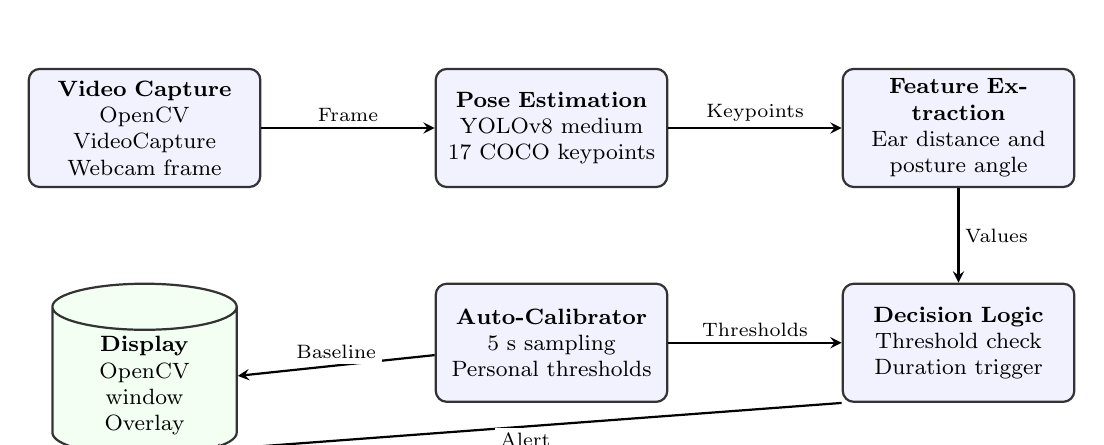
\begin{tikzpicture}[
        node distance=2.2cm, auto,
        block/.style={rectangle, draw=black!80, thick, fill=blue!5,
            text width=2.8cm, text centered, rounded corners, minimum height=1.5cm,
            inner sep=2pt, font=\footnotesize},
        db/.style={cylinder, draw=black!80, thick, fill=green!5,
            shape border rotate=90, aspect=0.25, text width=2.2cm, text centered,
            minimum height=1.6cm, inner sep=2pt, font=\footnotesize},
        flow/.style={draw, thick, ->, >=stealth},
        lbl/.style={font=\scriptsize, fill=white, inner sep=2pt, align=center}
    ]
    \node [block] (webcam) {\textbf{Video Capture}\\ OpenCV VideoCapture\\ Webcam frame};
    \node [block, right=of webcam] (pose) {\textbf{Pose Estimation}\\ YOLOv8 medium\\ 17 COCO keypoints};
    \node [block, right=of pose] (features) {\textbf{Feature Extraction}\\ Ear distance and\\ posture angle};
    \node [block, below=1.2cm of features] (decision) {\textbf{Decision Logic}\\ Threshold check\\ Duration trigger};
    \node [block, below=1.2cm of pose] (calibration) {\textbf{Auto-Calibrator}\\ 5 s sampling\\ Personal thresholds};
    \node [db, below=1.2cm of webcam] (display) {\textbf{Display}\\ OpenCV window\\ Overlay};

    \draw [flow] (webcam) -- node[above, lbl] {Frame} (pose);
    \draw [flow] (pose) -- node[above, lbl] {Keypoints} (features);
    \draw [flow] (features) -- node[right, lbl] {Values} (decision);
    \draw [flow] (calibration) -- node[above, lbl] {Thresholds} (decision);
    \draw [flow] (decision.south west) -- node[below, lbl] {Alert} (display.south east);
    \draw [flow] (calibration) -- node[above, lbl] {Baseline} (display);
    \end{tikzpicture}%
    }
    \caption{System architecture}
    \label{fig:arch_diagram}
\end{figure}

\subsection{High Level Design}
Figure~\ref{fig:flow} shows the flow of the main loop and Table~\ref{tab:modules} lists the
modules.

\begin{figure}[htpb]
    \centering
    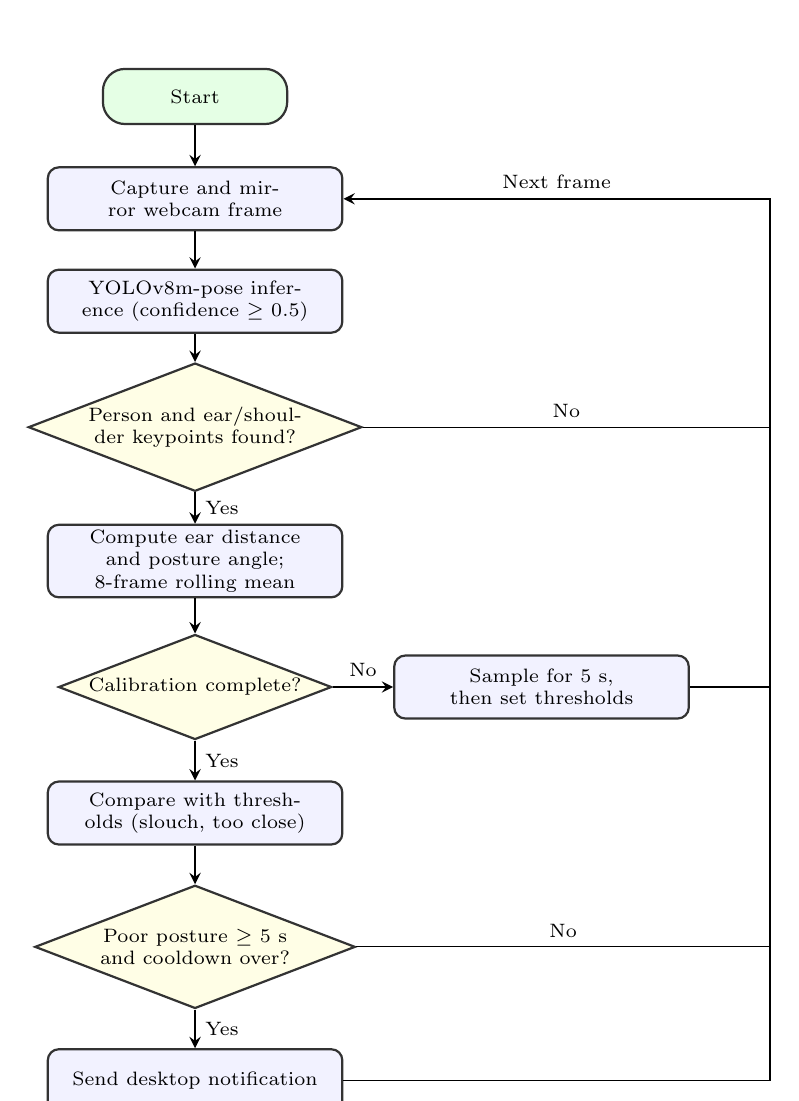
\begin{tikzpicture}[
        font=\scriptsize,
        proc/.style={rectangle, draw=black!80, thick, fill=blue!5, rounded corners,
            text width=3.6cm, align=center, minimum height=0.8cm, inner sep=2pt},
        term/.style={rectangle, draw=black!80, thick, fill=green!10, rounded corners=8pt,
            text width=2.2cm, align=center, minimum height=0.7cm, inner sep=2pt},
        dec/.style={diamond, aspect=2.6, draw=black!80, thick, fill=yellow!10,
            text width=2.9cm, align=center, inner sep=0pt},
        arr/.style={->, >=stealth, thick}
    ]
    \node[term] (start) at (0,0) {Start};
    \node[proc] (cap)   at (0,-1.3) {Capture and mirror webcam frame};
    \node[proc] (inf)   at (0,-2.6) {YOLOv8m-pose inference (confidence $\geq$ 0.5)};
    \node[dec]  (valid) at (0,-4.2) {Person and ear/shoulder keypoints found?};
    \node[proc] (calc)  at (0,-5.9) {Compute ear distance and posture angle; 8-frame rolling mean};
    \node[dec]  (cal)   at (0,-7.5) {Calibration complete?};
    \node[proc] (samp)  at (4.4,-7.5) {Sample for 5 s, then set thresholds};
    \node[proc] (cmp)   at (0,-9.1) {Compare with thresholds (slouch, too close)};
    \node[dec]  (bad)   at (0,-10.8) {Poor posture $\geq$ 5 s and cooldown over?};
    \node[proc] (notif) at (0,-12.5) {Send desktop notification};
    \coordinate (L) at (7.3,0);

    \draw[arr] (start) -- (cap);
    \draw[arr] (cap) -- (inf);
    \draw[arr] (inf) -- (valid);
    \draw[arr] (valid) -- node[right]{Yes} (calc);
    \draw[arr] (calc) -- (cal);
    \draw[arr] (cal) -- node[right]{Yes} (cmp);
    \draw[arr] (cmp) -- (bad);
    \draw[arr] (bad) -- node[right]{Yes} (notif);
    \draw[arr] (cal) -- node[above]{No} (samp);

    \draw (valid.east) -- node[above]{No} (L |- valid.east);
    \draw (samp.east) -- (L |- samp.east);
    \draw (bad.east) -- node[above]{No} (L |- bad.east);
    \draw (notif.east) -- (L |- notif.east);
    \draw[arr] (L |- notif.east) -- (L |- cap.east) -- node[above]{Next frame} (cap.east);
    \end{tikzpicture}
    \caption{Flowchart of the monitoring loop}
    \label{fig:flow}
\end{figure}

\begin{table}[htpb]
\centering
\caption{Main modules}\label{tab:modules}
\renewcommand{\arraystretch}{1.25}
\begin{tabularx}{\textwidth}{@{}>{\raggedright\arraybackslash}p{3.6cm}Y@{}}
\toprule
\textbf{Module} & \textbf{Job}\\
\midrule
Capture & Reads frames from the webcam and mirrors them.\\
Pose estimator & Loads \texttt{yolov8m-pose.pt} once and returns keypoints for each frame.\\
\texttt{calculate\_angle} & Gives the angle at a vertex formed by three points.\\
\texttt{AutoCalibrator} & Collects samples for 5 s and sets the personal thresholds.\\
Smoothing buffers & Two buffers of length 8 holding recent distances and angles.\\
Alert logic & Keeps the bad-posture timer and the cooldown, and calls Plyer.\\
Overlay and controls & Draws text and markers with OpenCV and reads key presses.\\
\bottomrule
\end{tabularx}
\end{table}

\subsection{Detailed Design}

\subsubsection{Keypoints and measurements}
Of the 17 COCO keypoints we use four: left ear (3), right ear (4), left shoulder (5) and
right shoulder (6). They are usually visible for a person facing the screen and are more
stable than points lower on the body. Figure~\ref{fig:keypoints} shows the points and the
angle.

\begin{figure}[htpb]
    \centering
    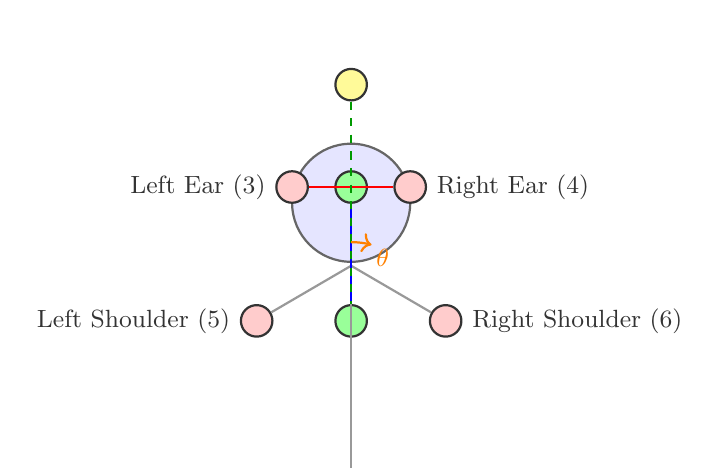
\begin{tikzpicture}[
        kp/.style={circle, draw=black!80, thick, fill=red!20, minimum size=0.4cm,
            inner sep=0pt, font=\scriptsize},
        lab/.style={font=\small, text=black!80}
    ]
    \node[circle, draw=black!60, thick, fill=blue!10, minimum size=1.5cm] (head) at (0,4) {};
    \node[kp, label={[lab]left:Left Ear (3)}]  (lear) at (-0.75,4.2) {};
    \node[kp, label={[lab]right:Right Ear (4)}] (rear) at (0.75,4.2) {};
    \node[kp, label={[lab]left:Left Shoulder (5)}]  (lsh) at (-1.2,2.5) {};
    \node[kp, label={[lab]right:Right Shoulder (6)}] (rsh) at (1.2,2.5) {};
    \node[kp, fill=green!40] (midear) at (0,4.2) {};
    \node[kp, fill=green!40] (midsh) at (0,2.5) {};
    \node[kp, fill=yellow!40] (refvert) at (0,5.5) {};
    \draw[black!40, thick] (head) -- (0,3.2);
    \draw[black!40, thick] (0,3.2) -- (lsh);
    \draw[black!40, thick] (0,3.2) -- (rsh);
    \draw[black!40, thick] (0,3.2) -- (0,0.5);
    \draw[red, thick] (lear) -- (rear);
    \draw[blue, thick] (midear) -- (midsh);
    \draw[green!60!black, dashed, thick] (refvert) -- (midsh);
    \draw[orange, thick, ->] (0,3.5) arc (90:75:1);
    \node[font=\small, text=orange] at (0.4,3.3) {$\theta$};
    \end{tikzpicture}
    \caption{Keypoints and posture angle}
    \label{fig:keypoints}
\end{figure}

The \textbf{inter-ear distance} is the straight-line distance between the two ears,
\begin{equation}
d = \sqrt{(x_{R}-x_{L})^{2} + (y_{R}-y_{L})^{2}}.
\end{equation}
The closer the user sits to the camera, the larger $d$ is in pixels, so it works as a
simple measure of distance from the screen. The \textbf{posture angle} $\theta$ is the
angle at the mid-point of the shoulders $B$, between a point $A=(x_B,0)$ straight above it
and the mid-point of the ears $C$:
\begin{equation}
\theta = \left|\arctan2(C_y-B_y,\,C_x-B_x)-\arctan2(A_y-B_y,\,A_x-B_x)\right|\times\frac{180}{\pi},
\end{equation}
and if $\theta>180^\circ$ we use $360^\circ-\theta$.

\begin{lstlisting}[language=Python, caption={Angle and feature computation}, label=lst:features]
def calculate_angle(a, b, c):
    a, b, c = np.array(a), np.array(b), np.array(c)
    radians = np.arctan2(c[1]-b[1], c[0]-b[0]) - np.arctan2(a[1]-b[1], a[0]-b[0])
    angle = np.abs(radians * 180.0 / np.pi)
    if angle > 180.0:
        angle = 360 - angle
    return angle

raw_ear_dist = math.hypot(r_ear[0]-l_ear[0], r_ear[1]-l_ear[1])
mid_ear      = [(l_ear[0]+r_ear[0])/2, (l_ear[1]+r_ear[1])/2]
mid_shoulder = [(l_shoulder[0]+r_shoulder[0])/2, (l_shoulder[1]+r_shoulder[1])/2]
reference_vertical = [mid_shoulder[0], 0]
raw_posture_angle = calculate_angle(reference_vertical, mid_shoulder, mid_ear)
\end{lstlisting}

\subsubsection{Checking the detection}
A frame is used only if the model returns at least seven keypoints and the x-coordinates of
both ears and both shoulders are above zero, because the model gives zero for points it
cannot find. Only the first detected person is used.

\subsubsection{Smoothing}
The distance and angle of each valid frame go into two buffers that hold the last 8 values.
All later steps use the mean of these buffers. This removes single-frame jitter and adds a
small delay of about eight frames, roughly one second at 8 FPS.

\subsubsection{Calibration}
The \texttt{AutoCalibrator} class works in two steps.
\begin{enumerate}
    \item \textbf{Sampling (5 s):} while the user sits in a good posture, the smoothed
          distance and angle of every frame are stored and a countdown is shown.
    \item \textbf{Thresholds:} the baselines $\bar d$ and $\bar\theta$ are the averages of
          the samples, and the thresholds are
          \begin{equation}
          T_{close} = 1.20\,\bar d, \qquad T_{slouch} = \bar\theta - 12^\circ .
          \end{equation}
\end{enumerate}
Pressing \texttt{c} starts calibration again, for example after moving the chair or the
camera. If no valid samples were collected, calibration restarts by itself.

\begin{lstlisting}[language=Python, caption={Threshold calculation in AutoCalibrator}, label=lst:calibration]
if elapsed < self.duration:
    self.dist_samples.append(current_dist)
    self.angle_samples.append(current_angle)
    return False, f"CALIBRATING... Sit straight! ({time_left}s)"
else:
    base_dist  = sum(self.dist_samples)  / len(self.dist_samples)
    base_angle = sum(self.angle_samples) / len(self.angle_samples)
    self.too_close_thresh = base_dist * 1.20
    self.slouch_thresh    = base_angle - 12.0
    self.is_calibrated = True
\end{lstlisting}

\subsubsection{Detection and alerts}
After calibration a frame counts as poor posture if
\[
d_{smooth} > T_{close} \quad\text{or}\quad \theta_{smooth} < T_{slouch}.
\]
When poor posture first appears, a timer starts. If it lasts for at least
\texttt{SLOUCH\_TIME\_TRIGGER} = 5 s and at least \texttt{NOTIFICATION\_COOLDOWN} = 10 s
have passed since the last alert, a desktop notification titled ``Ergonomic Alert'' is sent
through Plyer. When the posture returns to normal the timer is reset. The timer is also
kept at zero while calibration is running.

\begin{lstlisting}[language=Python, caption={Alert logic}, label=lst:alert]
is_too_close = ear_distance  > calibrator.too_close_thresh
is_slouching = posture_angle < calibrator.slouch_thresh

if is_slouching or is_too_close:
    if slouch_start_time is None:
        slouch_start_time = current_time
    slouch_duration = current_time - slouch_start_time
    if slouch_duration >= SLOUCH_TIME_TRIGGER:
        if current_time - last_notification_time > NOTIFICATION_COOLDOWN:
            notification.notify(title="Ergonomic Alert",
                message="You have been slouching ... Sit up straight.",
                app_name="Posture Monitor", timeout=4)
            last_notification_time = current_time
else:
    slouch_start_time = None
\end{lstlisting}

\subsubsection{Overlay and controls}
The overlay marks the mid-ear with a blue circle and the mid-shoulder with a green circle
and joins them with a yellow line. During calibration an orange banner counts down the
time. Afterwards the smoothed ear distance and posture angle are printed with their
thresholds, and a red counter shows how long bad posture has lasted. The keys \texttt{c}
and \texttt{q} recalibrate and quit.

\subsection{Dataset Description}
We did not collect a dataset or train any model. The pose model is the pre-trained
\texttt{yolov8m-pose.pt} checkpoint (about 51~MB), which Ultralytics trained on the
\textbf{COCO Keypoints} dataset \cite{cocodataset}, a large collection of images of people
annotated with 17 body keypoints. While the program runs, its only input is the live
webcam video. Frames are processed in memory and then discarded. Table~\ref{tab:kp} lists
the keypoints we use.

\begin{table}[htpb]
\centering
\caption{COCO keypoints used}\label{tab:kp}
\renewcommand{\arraystretch}{1.2}
\begin{tabular}{@{}cll@{}}
\toprule
\textbf{Index} & \textbf{Body part} & \textbf{Used for}\\
\midrule
3 & Left ear & Ear distance, mid-ear\\
4 & Right ear & Ear distance, mid-ear\\
5 & Left shoulder & Mid-shoulder\\
6 & Right shoulder & Mid-shoulder\\
\bottomrule
\end{tabular}
\end{table}

\subsection{Tools and Technologies Used}
\begin{table}[htpb]
\centering
\caption{Tools and settings}\label{tab:tools}
\renewcommand{\arraystretch}{1.25}
\begin{tabularx}{\textwidth}{@{}>{\raggedright\arraybackslash}p{5cm}Y@{}}
\toprule
\textbf{Tool or setting} & \textbf{Details}\\
\midrule
Python 3.10+ & Programming language\\
Ultralytics YOLO v8, PyTorch & Pose inference and backend \cite{ultralytics,pytorch}\\
\texttt{yolov8m-pose.pt} & Pre-trained medium pose model, 51 MB\\
OpenCV & Video capture, drawing and display \cite{opencv}\\
NumPy & Arrays and angle calculation\\
Plyer & Desktop notifications \cite{plyer}\\
Detection confidence & 0.5\\
Calibration time & 5 s\\
Smoothing window & 8 frames\\
Too-close threshold & 120\% of the baseline ear distance\\
Slouch threshold & Baseline angle $-12^\circ$\\
Alert trigger and cooldown & 5 s and 10 s\\
\bottomrule
\end{tabularx}
\end{table}

\clearpage
\section{Results and Discussion}

\subsection{Experimentation Environment Set-up}
The program was run in a Python virtual environment on a Windows laptop using its built-in
webcam, with one user sitting in front of the screen in normal indoor light
(Table~\ref{tab:env}).

\begin{table}[htpb]
\centering
\caption{Experimental environment}\label{tab:env}
\renewcommand{\arraystretch}{1.25}
\begin{tabularx}{\textwidth}{@{}>{\raggedright\arraybackslash}p{4.5cm}Y@{}}
\toprule
\textbf{Item} & \textbf{Details}\\
\midrule
Operating system & Windows\\
Processor, GPU, RAM & Intel Core i5-1135G7, Intel Iris Xe (integrated), 8 GB RAM\\
Camera & Built-in HD webcam, 1280 $\times$ 720 at 30 FPS\\
Software & Python, Ultralytics, PyTorch, OpenCV, NumPy, Plyer\\
Model & \texttt{yolov8m-pose.pt}, confidence 0.5\\
\bottomrule
\end{tabularx}
\end{table}

\subsection{Functional Requirements Results Achieved}
All the functional requirements in Table~\ref{tab:fr} are implemented in \texttt{main.py}.
Table~\ref{tab:frres} lists how each was exercised and what the program does.

\begin{table}[htpb]
\centering
\caption{Functional requirement results}\label{tab:frres}
\footnotesize
\renewcommand{\arraystretch}{1.25}
\begin{tabularx}{\textwidth}{@{}l>{\raggedright\arraybackslash}p{3.4cm}Yl@{}}
\toprule
\textbf{ID} & \textbf{Test} & \textbf{Behaviour} & \textbf{Status}\\
\midrule
FR1, FR2 & Start the program & A mirrored webcam window opens and keypoints are found in every frame & Done\\
FR3 & Cover an ear or leave the frame & The frame is skipped and the program keeps running & Done\\
FR4, FR5 & Sit still in front of the camera & Ear distance and angle are shown as steady values & Done\\
FR6 & Sit upright for the first 5 s & A countdown banner shows, then the thresholds appear & Done\\
FR7 & Lean towards the screen or slouch & A value crosses its threshold and the bad-posture counter starts & Done\\
FR8 & Keep bad posture for over 5 s & A notification appears, alerts are at least 10 s apart, and the timer resets on correction & Done\\
FR9 & Watch the window & Circles, line, values, thresholds and counter are drawn & Done\\
FR10 & Press \texttt{c} and \texttt{q} & Calibration restarts, and the program closes & Done\\
\bottomrule
\end{tabularx}
\end{table}

Figure~\ref{fig:timeline} shows how the alert logic behaves over time. If bad posture
continues, the first alert comes after 5 s and the next one after the 10 s cooldown. A
short lapse of less than 5 s gives no alert at all, which is how the system avoids
nagging the user.

\begin{figure}[htpb]
    \centering
    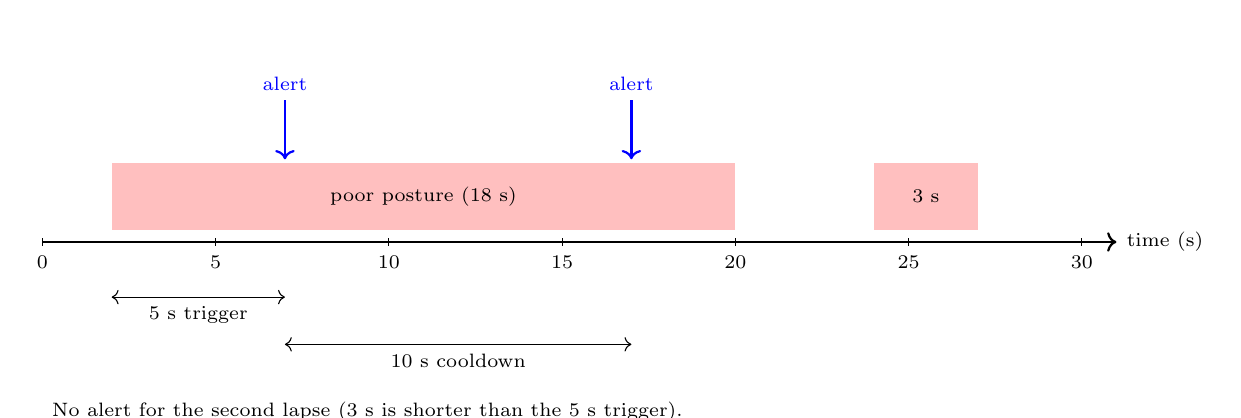
\begin{tikzpicture}[x=0.44cm, y=0.5cm, font=\scriptsize]
        \draw[->, thick] (0,0) -- (31,0) node[right]{time (s)};
        \foreach \t in {0,5,10,15,20,25,30} {\draw (\t,0.1) -- (\t,-0.1) node[below]{\t};}
        \fill[red!25] (2,0.3) rectangle (20,2);
        \fill[red!25] (24,0.3) rectangle (27,2);
        \node at (11,1.15) {poor posture (18 s)};
        \node at (25.5,1.15) {3 s};
        \foreach \t in {7,17} {
            \draw[blue, thick, ->] (\t,3.6) -- (\t,2.1);
            \node[blue, above] at (\t,3.6) {alert};
        }
        \draw[<->] (2,-1.4) -- node[below]{5 s trigger} (7,-1.4);
        \draw[<->] (7,-2.6) -- node[below]{10 s cooldown} (17,-2.6);
        \node[align=left, anchor=west] at (0,-4.3) {No alert for the second lapse (3 s is shorter than the 5 s trigger).};
    \end{tikzpicture}
    \caption{Example timeline of the duration trigger and cooldown}
    \label{fig:timeline}
\end{figure}

\subsection{Non-Functional Requirements Results Achieved}
Table~\ref{tab:nfrres} gives the non-functional results. The timing values follow from the
settings of the program, and the run-time figures depend on the laptop used.

\begin{table}[htpb]
\centering
\caption{Non-functional requirement results}\label{tab:nfrres}
\footnotesize
\renewcommand{\arraystretch}{1.25}
\begin{tabularx}{\textwidth}{@{}>{\raggedright\arraybackslash}p{3.3cm}>{\raggedright\arraybackslash}p{4.4cm}Y@{}}
\toprule
\textbf{Attribute} & \textbf{Result} & \textbf{Remark}\\
\midrule
Frame rate & About 8 FPS & Average over a one-minute run with the user in frame\\
Time per frame & About 125 ms & Capture, inference and drawing\\
CPU and RAM use & About 70\% CPU, 2.0 GB RAM & Read from the task manager\\
Smoothing delay & 8 frames (about 1 s at 8 FPS) & Caused by the rolling mean\\
Calibration time & 5 s & Fixed sampling window\\
Alert delay & At least 5 s of bad posture & Duration trigger\\
Alert rate & At most one in 10 s & Cooldown\\
Model size & 51 MB & \texttt{yolov8m-pose.pt}\\
Extra hardware & None & Only a webcam\\
Privacy & Local processing & No video is saved or sent\\
\bottomrule
\end{tabularx}
\end{table}

\subsection{Comparison of Results with Existing Works}
The papers we reviewed use different sensors, tasks and datasets, and our project uses a
pre-trained model with rule-based thresholds and not a newly trained classifier, so their
accuracy figures cannot be compared with ours directly. Table~\ref{tab:compare} therefore
compares the approaches.

\begin{table}[htpb]
\centering
\caption{Comparison with existing work}\label{tab:compare}
\footnotesize
\renewcommand{\arraystretch}{1.25}
\begin{tabularx}{\textwidth}{@{}>{\raggedright\arraybackslash}p{3.3cm}>{\raggedright\arraybackslash}p{2.5cm}>{\raggedright\arraybackslash}p{3.6cm}Y@{}}
\toprule
\textbf{Work} & \textbf{Sensor} & \textbf{Approach} & \textbf{Remark}\\
\midrule
Bourahmoune et al. \cite{bourahmoune2022cushion} & Pressure cushion & Machine learning on pressure data & Needs extra hardware\\
Wang et al. \cite{wang2025pressure} & Seat pressure & Deep learning on pressure maps & Needs extra hardware\\
Cao et al. \cite{cao2025keypointnet} & Camera & Keypoint-based network, several views & Focus on the recognition model\\
Zhu and Wu \cite{zhu2025rtmposelrf} & Camera & RTMPose-based recognition & Focus on the recognition model\\
Seo and Lee \cite{seo2021automated}, Lee and Lee \cite{lee2022see} & Camera & Posture classification and risk assessment & Industrial and construction work\\
Supanich et al. \cite{supanich2023mediapipe} & Webcam & MediaPipe Pose with ML & Exercise posture\\
\textbf{This work} & \textbf{Webcam} & \textbf{YOLOv8m-pose, geometry, calibration} & \textbf{Ready-to-use tool with personal thresholds, smoothing, delayed alerts and cooldown}\\
\bottomrule
\end{tabularx}
\end{table}

\textbf{Discussion.} Compared with sensor-based systems, ours needs nothing to be bought or
installed. Compared with the camera-based recognition models, it is simpler and easy to
explain: two measurements and thresholds taken from the user's own posture, with no
classifier to train. Its limits are that it measures in pixels from a 2D image and expects
the user to face the camera, so thresholds are relative to the calibrated position and not
absolute. The slouch angle in particular depends on where the camera is placed, so the
user should calibrate from the normal camera position and recalibrate after moving it.

\subsection{Project GUI Snapshots}
The window shows the mirrored webcam feed with the overlay. Figures~\ref{fig:g1} to
\ref{fig:g4} show the main functions.

\begin{figure}[htpb]
\centering
\snap{images/gui_calibration.png}{Calibration banner with countdown}
\caption{Calibration with the countdown banner}\label{fig:g1}
\end{figure}

\begin{figure}[htpb]
\centering
\snap{images/gui_monitoring.png}{Good posture: keypoints, values and thresholds}
\caption{Monitoring with good posture}\label{fig:g2}
\end{figure}

\begin{figure}[htpb]
\centering
\snap{images/gui_badposture.png}{Bad posture counter in red}
\caption{Bad posture detected, with the duration counter}\label{fig:g3}
\end{figure}

\begin{figure}[htpb]
\centering
\snap{images/gui_notification.png}{Desktop notification ``Ergonomic Alert''}
\caption{Desktop notification after sustained bad posture}\label{fig:g4}
\end{figure}

\subsection{Societal Impact of the Project}
Bad sitting posture affects students, office staff and people working from home, and leads
to neck, shoulder and back problems and lost productivity. This tool gives anyone with a
webcam regular, personal posture feedback without buying a wearable or special furniture.
Because processing is local and no video is stored or sent, privacy is protected. Schools,
small companies and people with limited budgets can benefit the most. The project also shows
that a pre-trained AI model can be reused for a health-related task without collecting
data or training anything.

\subsection{SDG Mapped}
\begin{table}[htpb]
\centering
\caption{Sustainable Development Goals addressed}\label{tab:sdg}
\renewcommand{\arraystretch}{1.25}
\begin{tabularx}{\textwidth}{@{}>{\raggedright\arraybackslash}p{4.4cm}Y@{}}
\toprule
\textbf{SDG} & \textbf{Contribution}\\
\midrule
SDG 3: Good Health and Well-being & Early reminders help prevent posture-related pain and injury.\\
SDG 9: Industry, Innovation and Infrastructure & Applies an existing AI model to a new practical problem on common hardware.\\
SDG 10: Reduced Inequalities & Free software that does not depend on being able to buy extra hardware.\\
\bottomrule
\end{tabularx}
\end{table}

\clearpage
\section*{Conclusion and Future Scope}
\addcontentsline{toc}{section}{Conclusion and Future Scope}

\textbf{Conclusion.} We built the Touchless Ergonomic Posture Monitor, which uses the YOLOv8
medium pose model and a normal webcam to detect slouching and sitting too close to the
screen. It computes the ear distance and posture angle from four keypoints, smooths them
over 8 frames, and compares them with thresholds set for the user in a five-second
calibration. Alerts are sent only after bad posture lasts five seconds and are limited by a
cooldown, and a live overlay shows what the system is doing. The project shows that a
pre-trained pose model together with simple logic can give useful posture feedback at
almost no cost, and keeps the video on the user's own computer. Along the way we learned
about pose estimation, working with keypoints, smoothing, building real-time interfaces
with OpenCV, and writing technical reports.

\textbf{Limitations.} The system handles one person, expects the camera to face the user
roughly from the front, depends on good lighting, measures in pixels and not real
distance, and looks only at the upper body. It also cannot tell when the user has left
the seat.

\textbf{Future scope.}
\begin{itemize}
    \item Support for several people in the frame.
    \item Saving posture data and showing daily or weekly reports.
    \item Optional sound alerts and break reminders.
    \item Detecting forward head tilt (``tech neck'').
    \item Better distance estimation using a depth camera.
    \item A settings screen for sensitivity, calibration time and thresholds.
    \item Testing against labelled sitting-posture data and trying lighter models for
          low-power devices.
    \item A phone app for viewing posture reports.
\end{itemize}

\clearpage
\section*{References}
\addcontentsline{toc}{section}{References}
\begingroup
\small
\setstretch{1.15}
\begin{thebibliography}{99}
\setlength{\itemsep}{3pt}

\bibitem{mcfarlane2002scope}
D. C. McFarlane and K. A. Latorella, ``The scope and importance of human interruption in human-computer interaction design,'' \textit{Human--Computer Interaction}, vol. 17, no. 1, pp. 1--61, 2002.

\bibitem{deeppose}
A. Toshev and C. Szegedy, ``DeepPose: Human pose estimation via deep neural networks,'' in \textit{Proc. IEEE Conf. Computer Vision and Pattern Recognition (CVPR)}, 2014, pp. 1653--1660.

\bibitem{tompson2014joint}
J. Tompson, A. Jain, Y. LeCun and C. Bregler, ``Joint training of a convolutional network and a graphical model for human pose estimation,'' in \textit{Advances in Neural Information Processing Systems (NeurIPS)}, vol. 27, 2014, pp. 1799--1807.

\bibitem{cocodataset}
T.-Y. Lin \textit{et al.}, ``Microsoft COCO: Common objects in context,'' in \textit{Proc. European Conf. Computer Vision (ECCV)}, 2014, pp. 740--755.

\bibitem{redmon2016you}
J. Redmon, S. Divvala, R. Girshick and A. Farhadi, ``You only look once: Unified, real-time object detection,'' in \textit{Proc. IEEE CVPR}, 2016, pp. 779--788.

\bibitem{lugaresi2019mediapipe}
C. Lugaresi \textit{et al.}, ``MediaPipe: A framework for building perception pipelines,'' \textit{arXiv:1906.08172}, 2019.

\bibitem{hrnet}
K. Sun, B. Xiao, D. Liu and J. Wang, ``Deep high-resolution representation learning for human pose estimation,'' in \textit{Proc. IEEE/CVF CVPR}, 2019, pp. 5693--5703.

\bibitem{blazepose}
V. Bazarevsky \textit{et al.}, ``BlazePose: On-device real-time body pose tracking,'' \textit{arXiv:2006.10204}, 2020.

\bibitem{openpose}
Z. Cao, G. Hidalgo, T. Simon, S.-E. Wei and Y. Sheikh, ``OpenPose: Realtime multi-person 2D pose estimation using part affinity fields,'' \textit{IEEE Trans. Pattern Analysis and Machine Intelligence}, vol. 43, no. 1, pp. 172--186, 2021.

\bibitem{seo2021automated}
J. Seo and S. Lee, ``Automated postural ergonomic risk assessment using vision-based posture classification,'' \textit{Automation in Construction}, vol. 128, p. 103725, 2021.

\bibitem{maji2022yolopose}
D. Maji, S. Nagori, M. Mathew and D. Poddar, ``YOLO-Pose: Enhancing YOLO for multi person pose estimation using object keypoint similarity loss,'' in \textit{Proc. IEEE/CVF CVPR Workshops}, 2022, pp. 2637--2646.

\bibitem{vitpose}
Y. Xu, J. Zhang, Q. Zhang and D. Tao, ``ViTPose: Simple vision transformer baselines for human pose estimation,'' in \textit{Advances in Neural Information Processing Systems (NeurIPS)}, vol. 35, 2022, pp. 38571--38584.

\bibitem{lee2022see}
Y.-C. Lee and C.-H. Lee, ``SEE: A proactive strategy-centric and deep learning-based ergonomic risk assessment system for risky posture recognition,'' \textit{Advanced Engineering Informatics}, vol. 53, p. 101717, 2022.

\bibitem{bourahmoune2022cushion}
K. Bourahmoune, K. Ishac and T. Amagasa, ``Intelligent posture training: Machine-learning-powered human sitting posture recognition based on a pressure-sensing IoT cushion,'' \textit{Sensors}, vol. 22, no. 14, p. 5337, 2022.

\bibitem{gamra2022yopose}
M. Ben Gamra and M. A. Akhloufi, ``YoPose: Yoga posture recognition using deep pose estimation,'' in \textit{Proc. 3rd Int. Conf. Human-Centric Smart Environments for Health and Well-being (IHSH)}, 2022, pp. 88--93.

\bibitem{amadi2023postureposE}
L. Amadi and G. Agam, ``PosturePose: Optimized posture analysis for semi-supervised monocular 3D human pose estimation,'' \textit{Sensors}, vol. 23, no. 24, p. 9749, 2023.

\bibitem{wang2023yolov7}
C.-Y. Wang, A. Bochkovskiy and H.-Y. M. Liao, ``YOLOv7: Trainable bag-of-freebies sets new state-of-the-art for real-time object detectors,'' in \textit{Proc. IEEE/CVF CVPR}, 2023, pp. 7464--7475.

\bibitem{terven2023yolo}
J. Terven, D.-M. C\'ordova-Esparza and J.-A. Romero-Gonz\'alez, ``A comprehensive review of YOLO architectures in computer vision: From YOLOv1 to YOLOv8 and YOLO-NAS,'' \textit{Machine Learning and Knowledge Extraction}, vol. 5, no. 4, pp. 1680--1716, 2023.

\bibitem{zheng2023survey}
C. Zheng \textit{et al.}, ``Deep learning-based human pose estimation: A survey,'' \textit{ACM Computing Surveys}, vol. 56, no. 1, Art. 11, 2023.

\bibitem{jiang2023rtmpose}
T. Jiang \textit{et al.}, ``RTMPose: Real-time multi-person pose estimation based on MMPose,'' \textit{arXiv:2303.07399}, 2023.

\bibitem{supanich2023mediapipe}
W. Supanich, S. Kulkarineetham, P. Sukphokha and P. Wisarnsart, ``Machine learning-based exercise posture recognition system using MediaPipe pose estimation framework,'' in \textit{Proc. 9th Int. Conf. Advanced Computing and Communication Systems (ICACCS)}, 2023, pp. 2003--2007.

\bibitem{ding2024yolopose}
J. Ding, S. Niu and Z. Nie, ``Research on human posture estimation algorithm based on YOLO-Pose,'' \textit{Sensors}, vol. 24, no. 10, p. 3036, 2024.

\bibitem{lu2024ksl}
T. Lu, K. Cheng and X. Hua, ``KSL-POSE: A real-time 2D human pose estimation method based on modified YOLOv8-Pose framework,'' \textit{Sensors}, vol. 24, no. 19, p. 6249, 2024.

\bibitem{yang2024review}
Z. Yang, D. Song, J. Ning and Z. Wu, ``A systematic review: Advancing ergonomic posture risk assessment through the integration of computer vision and machine learning techniques,'' \textit{IEEE Access}, vol. 12, pp. 180481--180519, 2024.

\bibitem{cao2025keypointnet}
Z. Cao, X. Wu, C. Wu, S. Jiao, Y. Xiao, Y. Zhang and Y. Zhou, ``KeypointNet: An efficient deep learning model with multi-view recognition capability for sitting posture recognition,'' \textit{Electronics}, vol. 14, no. 4, p. 718, 2025.

\bibitem{zhu2025rtmposelrf}
H. Zhu and M. Wu, ``RTMPose-LRF: Real-time pose estimation method for sitting posture recognition,'' in \textit{Proc. 7th Int. Conf. Internet of Things, Automation and Artificial Intelligence (IoTAAI)}, 2025, pp. 276--279.

\bibitem{liu2025yolov11}
J. Liu and J. Qiu, ``Improved lightweight human posture recognition based on YOLOv11-Pose,'' in \textit{Proc. 6th Int. Conf. Computer Vision, Image and Deep Learning (CVIDL)}, 2025, pp. 1169--1172.

\bibitem{wang2025pressure}
B. Wang, L. Tu, Q.-Q. Shi and S. Mo, ``Deep learning-based sitting posture recognition from pressure distribution across hard and soft seat environment,'' \textit{Applied Sciences}, vol. 15, no. 23, p. 12744, 2025.

\bibitem{wu2025badminton}
Y. Wu, Z. Chen and H. Zhang, ``Enhanced pose estimation for badminton players via improved YOLOv8-Pose with efficient local attention,'' \textit{Sensors}, vol. 25, no. 14, p. 4446, 2025.

\bibitem{xu2025simdlka}
X. Xu, T. Wu and Z. Du, ``Enhanced human pose estimation using YOLOv8 with integrated SimDLKA attention mechanism and DCIOU loss function: Analysis of human body behavior and posture,'' \textit{PLOS ONE}, vol. 20, no. 5, p. e0318578, 2025.

\bibitem{shanmugam2025sedentary}
D. B. Shanmugam and J. Dhilipan, ``Real-time posture monitoring prediction for mitigating sedentary health risks using deep learning techniques,'' \textit{Int. J. Informatics and Communication Technology (IJ-ICT)}, vol. 14, no. 3, pp. 1126--1135, 2025.

\bibitem{sharma2025cervical}
V. Sharma and V. Mohan K, ``Review on design of real-time posture monitoring system for the cervical region,'' \textit{Ergonomics}, vol. 68, no. 4, pp. 471--483, 2025.

\bibitem{ultralytics}
G. Jocher, A. Chaurasia and J. Qiu, ``Ultralytics YOLOv8,'' 2023. [Online]. Available: \url{https://github.com/ultralytics/ultralytics}

\bibitem{pytorch}
A. Paszke \textit{et al.}, ``PyTorch: An imperative style, high-performance deep learning library,'' in \textit{Advances in Neural Information Processing Systems (NeurIPS)}, vol. 32, 2019, pp. 8024--8035.

\bibitem{opencv}
G. Bradski, ``The OpenCV library,'' \textit{Dr. Dobb's Journal of Software Tools}, vol. 25, no. 11, pp. 120--125, 2000.

\bibitem{plyer}
Kivy Organization, ``Plyer: A Python library for accessing features of your hardware and platform.'' [Online]. Available: \url{https://plyer.readthedocs.io/}

\end{thebibliography}
\endgroup

\end{document}




